%%%%%%%%%%%%%%%%%%%%%%%%%
\section{Introduction}
\label{sec:Introduction}
%%%%%%%%%%%%%%%%%%%%%%%%%


Modular self-reconfigurable robots have been proposed as one method to create general purpose robots or arbitrary complexity in an autonomous way. These robots generally can be thought of as consisting of individual \textbf{modules}, which connect to other elements, either powered modules or passive structural elements, through standardized \textbf{connectors} to create a specific \textbf{configurations} in order to accomplish a designated task. Aside from their fundamental requirement of providing robust mechanical links, these connectors have been used in the literature to enable inter-module communication \cite{liedke2013collective} \cite{TosunDaveyLiuYim-IROS2016}, deliver power to modules \cite{todo} \cite{todo}, and determine the presence and relative orientation of adjacent units. While all of these improvements to inter-module connections are extensively explored by other researchers, solutions for gathering information about units are limited, and generally require both units to be active.  This paper focuses on this feature of connectors, looks at an overview of how location and identity information is encoded in connectors, and proposes a new method which the authors believe compares favorably with the existing state of the art.


For modular robots, knowing which neighbors they are connected to and the orientation in which they are connected facilitates solutions to the self-reconfiguration problem \cite{AHMADZADEH201527} \cite{surveyyim}. While some work has left this question unaddressed \cite{Neubert2016}, other authors use inter-module communication between modules to implicitly sense adjacent neighbors \cite{liedke2013collective} \cite{Gilpin-Thesis06} \cite{TosunDaveyLiuYim-IROS2016}.  Other systems use RFID tags \cite{Werfel-PhDThesis06} to explicitly sense module adjacency.  None of these methods allow modules to determine their relative rotational orientation to each other, and the majority require power and computational circuitry to determine adjacency, limiting the inclusion of ``passive'' modules in the robot as described by \cite{roombots5}.  Our new method for estimating the position of adjacent modules addresses both of these issues.  We introduce \tagNamePlural, arrangements of magnets mounted on the faces of modules.  The orientation of magnets which comprise \tagNamePlural can be measured by commodity encoder sensors, thereby reading information encoded in the orientation of the magnets.


The remainder of the paper is organized as follows:
Section~\ref{sec:RelatedWork} gives an overview of related
work that pertains to modular robots, and specifically to identifying and encoding physical location information in modular connectors.
Section~\ref{sec:Hardware} presents a quick overview of the 3D Mblock modules, and then gives a detailed description of the new magnetic tag hardware and electronics.
%Next Section ~\ref{sec:Algorithims} presents the two algorithms which utilize the magnetic tags to 1. turn arbitrary configurations into %a line, and 2. form simple shapes from a line of modules.
Next, Section~\ref{sec:Experiments}
presents data characterizing the hardware and the results of
experiments with the system.
Finally, Section~\ref{sec:Discussion}
concludes with a short discussion and ideas for future work.

\begin{figure}[t]
	\centering
	\begin{subfigure}[b]{1.75 in}
	%	\resizebox{.48\linewidth}{0.6 in}
	%	{
			\includegraphics[width=.9\linewidth]{Figures/mTagsCover.png}
	%	}
	%	\subcaption{b.}
	\end{subfigure}
	~
	\begin{subfigure}[b]{1.5 in}


		\resizebox{1.5 in}{1.25 in}
		{
			\begin{tikzpicture}[x=(220:1cm), y=(-40:1cm), z=(90:0.707cm)]
			%%
%this code is from...
\setcounter{x}{0}%
\setcounter{y}{0}%
\setcounter{z}{0}%

% The angles of x,y,z-axes
\newcommand\xaxis{210}
\newcommand\yaxis{-30}
\newcommand\zaxis{90}

% The top side of a cube
\newcommand\topside[3]{
	\fill[fill=yellow, draw=black,shift={(\xaxis:#1)},shift={(\yaxis:#2)},
	shift={(\zaxis:#3)}] (0,0) -- (30:1) -- (0,1) --(150:1)--(0,0);
}

% The left side of a cube
\newcommand\leftside[3]{
	\fill[fill=red, draw=black,shift={(\xaxis:#1)},shift={(\yaxis:#2)},
	shift={(\zaxis:#3)}] (0,0) -- (0,-1) -- (210:1) --(150:1)--(0,0);
}

% The right side of a cube
\newcommand\rightside[3]{
	\fill[fill=blue, draw=black,shift={(\xaxis:#1)},shift={(\yaxis:#2)},
	shift={(\zaxis:#3)}] (0,0) -- (30:1) -- (-30:1) --(0,-1)--(0,0);
}

% The cube 
\newcommand\cube[3]{
	\topside{#1}{#2}{#3} \leftside{#1}{#2}{#3} \rightside{#1}{#2}{#3}
}

\newcommand\ArrowNE[3]
{
	\node at (#1+0.5, #2+0.5, #3) 
%	\node at (#1, #2, #3) 
	{
		\begin{tikzpicture}
		\draw[->, thick, >={Stealth[round]}, line width=0.4mm] (0.3,0) -- (-0.3,0);
		\end{tikzpicture}};
		
}

\newcommand\ArrowNL[3]
{
	\node at (#1+1, #2+0.5, #3-0.5) 
	%	\node at (#1, #2, #3) 
	{
		\begin{tikzpicture}
		\draw[->, thick, >={Stealth[round]}, line width=0.4mm] (0.16,0.16) -- (-0.16,-0.16);
		\end{tikzpicture}};
	
}

\newcommand\ArrowNR[3]
{
	\node at (#1+0.5, #2+1, #3-0.5) 
	%	\node at (#1, #2, #3) 
	{
		\begin{tikzpicture}
		\draw[->, thick, >={Stealth[round]}, line width=0.4mm] (0.16,0.16) -- (-0.16,-0.16);
		\end{tikzpicture}};
	
}

\newcommand\ArrowNW[3]
{
	\node at (#1+0.5, #2+0.5, #3) 
%	\node at (#1, #2, #3) 
	{
		\begin{tikzpicture}
		\draw[->, thick, >={Stealth[round]}, line width=0.4mm] (0,0.3) -- (0,-0.3);
		\end{tikzpicture}};
	
}

\newcommand\ArrowSW[3]
{
	\node at (#1+0.5, #2+0.5, #3) 
%	\node at (#1, #2, #3) 
	{
		\begin{tikzpicture}
		\draw[<-, thick, >={Stealth[round]}, line width=0.4mm] (0.3,0) -- (-0.3,0);
		\end{tikzpicture}};
	
}

\newcommand\ArrowSE[3]
{
	\node at (#1+0.5, #2+0.5, #3) 
%	\node at (#1, #2, #3) 
	{
		\begin{tikzpicture}
		\draw[<-, thick, >={Stealth[round]}, line width=0.4mm] (0,0.3) -- (0,-0.3);
		\end{tikzpicture}};
	
}

% Definition of \planepartition
% To draw the following plane partition, just write \planepartition{ {a, b, c}, {d,e} }.
%  a b c
%  d e
\newcommand\planepartition[1]{
	\setcounter{x}{-1}
	\foreach \a in {#1} {
		\addtocounter{x}{1}
		\setcounter{y}{-1}
		\foreach \b in \a {
			\addtocounter{y}{1}
			\setcounter{z}{-1}
			\foreach \c in {0,...,\b} {
				\addtocounter{z}{1}
				\ifthenelse{\c=0}{\setcounter{z}{-1},\addtocounter{y}{0}}{
					\cube{\value{x}}{\value{y}}{\value{z}}}
			}
		}
	}
}


%%\begin{tikzpicture}[x=(220:1cm), y=(-40:1cm), z=(90:0.707cm)]
	%\planepartition{{0,0,1},{1,1,1},{1,0,0},{1,0,1}};
\foreach \m [count=\y] in {{1,1,1,1},{1,1,1},{1,1,1,1},{1,1,1}}{
	\foreach \n [count=\x] in \m {
		\ifnum \n>0
		\foreach \z in {1,...,\n}{
			\draw [fill=blue!30] (\x+1,\y,\z) -- (\x+1,\y+1,\z) -- (\x+1, \y+1, \z-1) -- (\x+1, \y, \z-1) -- cycle;
			\draw [fill=blue!40] (\x,\y+1,\z) -- (\x+1,\y+1,\z) -- (\x+1, \y+1, \z-1) -- (\x, \y+1, \z-1) -- cycle;
			\draw [fill=blue!10] (\x,\y,\z)   -- (\x+1,\y,\z)   -- (\x+1, \y+1, \z)   -- (\x, \y+1, \z) -- cycle;  
		}
	
		\fi
	}
}   

\foreach \m [count=\y] in {{0,0,0,1}, {0,0,0}} {
	\foreach \n [count=\x] in \m {
		\ifnum \n>0
		\foreach \z in {1,...,\n}{
			\draw [fill=green!30] (\x+1,\y,\z) -- (\x+1,\y+1,\z) -- (\x+1, \y+1, \z-1) -- (\x+1, \y, \z-1) -- cycle;
			\draw [fill=green!40] (\x,\y+1,\z) -- (\x+1,\y+1,\z) -- (\x+1, \y+1, \z-1) -- (\x, \y+1, \z-1) -- cycle;
			\draw [fill=green!10] (\x,\y,\z)   -- (\x+1,\y,\z)   -- (\x+1, \y+1, \z)   -- (\x, \y+1, \z) -- cycle;  
		}
		
		\fi
	}
}   

\ArrowNW{1}	{3}	{1};

\foreach \m [count=\y] in {{0,0,0,0},{0,0,0},{0,0,0,0},{2,0,0}}{
	\foreach \n [count=\x] in \m {
		\ifnum \n>0
		\foreach \z in {1,...,\n}{
			\draw [fill=orange!30] (\x+1,\y,\z) -- (\x+1,\y+1,\z) -- (\x+1, \y+1, \z-1) -- (\x+1, \y, \z-1) -- cycle;
			\draw [fill=orange!40] (\x,\y+1,\z) -- (\x+1,\y+1,\z) -- (\x+1, \y+1, \z-1) -- (\x, \y+1, \z-1) -- cycle;
			\draw [fill=orange!10] (\x,\y,\z)   -- (\x+1,\y,\z)   -- (\x+1, \y+1, \z)   -- (\x, \y+1, \z) -- cycle;  
		}
		
		\fi
	}
}  

\foreach \m [count=\y] in {{0},{0},{0},{0,1,1}}{
	\foreach \n [count=\x] in \m {
		\ifnum \n>0
		\foreach \z in {1,...,\n}{
			\draw [fill=blue!30] (\x+1,\y,\z) -- (\x+1,\y+1,\z) -- (\x+1, \y+1, \z-1) -- (\x+1, \y, \z-1) -- cycle;
			\draw [fill=blue!40] (\x,\y+1,\z) -- (\x+1,\y+1,\z) -- (\x+1, \y+1, \z-1) -- (\x, \y+1, \z-1) -- cycle;
			\draw [fill=blue!10] (\x,\y,\z)   -- (\x+1,\y,\z)   -- (\x+1, \y+1, \z)   -- (\x, \y+1, \z) -- cycle;  
		}
		
		\fi
	}
} 

\foreach \m [count=\y] in {{0},{0},{0},{1,0,0}}{
	\foreach \n [count=\x] in \m {
		\ifnum \n>0
		\foreach \z in {1,...,\n}{
		%	\draw [fill=blue!30] (\x+1,\y,\z) -- (\x+1,\y+1,\z) -- (\x+1, \y+1, \z-1) -- (\x+1, \y, \z-1) -- cycle;
			\draw [fill=blue!40] (\x,\y+1,\z) -- (\x+1,\y+1,\z) -- (\x+1, \y+1, \z-1) -- (\x, \y+1, \z-1) -- cycle;
		%	\draw [fill=blue!10] (\x,\y,\z)   -- (\x+1,\y,\z)   -- (\x+1, \y+1, \z)   -- (\x, \y+1, \z) -- cycle;  
		}
		
		\fi
	}
} 
		"x" "y" "z"

\ArrowNR{4} {1}	{1};
\ArrowNL{4} {1}	{1};

\ArrowNR{4} {3}	{1};
\ArrowNL{4} {3}	{1};

\ArrowNR{3} {4}	{1};
\ArrowNL{3} {4}	{1};

\ArrowNR{1} {4}	{1};
\ArrowNR{2} {4}	{1};

\ArrowNL{3} {2}	{1};

\ArrowSW{1}	{1}	{1};
\ArrowSW{2}	{1}	{1};
\ArrowSW{3}	{1}	{1};
\ArrowSW{4}	{1}	{1};


\ArrowNW{1}	{2}	{1};
\ArrowSW{2}	{2}	{1};
\ArrowNW{3}	{2}	{1};

\ArrowNW{2}	{3}	{1};
\ArrowNE{3}	{3}	{1};
\ArrowNE{4}	{3}	{1};

%\ArrowNW{1}	{4}	{1};
\ArrowSW{2}	{4}	{1};
\ArrowNW{3}	{4}	{1};

			\ArrowSW{4}{3}{2};

			\end{tikzpicture}
		}

		%	\subcaption{a.}
	\end{subfigure}


	\caption{\tagNamePlural renderings with displaying arrows}

	\label{fig:PlaneChanging2}
\end{figure}

%\begin{figure}[htb]
%
%	%%
%this code is from...
\setcounter{x}{0}%
\setcounter{y}{0}%
\setcounter{z}{0}%

% The angles of x,y,z-axes
\newcommand\xaxis{210}
\newcommand\yaxis{-30}
\newcommand\zaxis{90}

% The top side of a cube
\newcommand\topside[3]{
	\fill[fill=yellow, draw=black,shift={(\xaxis:#1)},shift={(\yaxis:#2)},
	shift={(\zaxis:#3)}] (0,0) -- (30:1) -- (0,1) --(150:1)--(0,0);
}

% The left side of a cube
\newcommand\leftside[3]{
	\fill[fill=red, draw=black,shift={(\xaxis:#1)},shift={(\yaxis:#2)},
	shift={(\zaxis:#3)}] (0,0) -- (0,-1) -- (210:1) --(150:1)--(0,0);
}

% The right side of a cube
\newcommand\rightside[3]{
	\fill[fill=blue, draw=black,shift={(\xaxis:#1)},shift={(\yaxis:#2)},
	shift={(\zaxis:#3)}] (0,0) -- (30:1) -- (-30:1) --(0,-1)--(0,0);
}

% The cube 
\newcommand\cube[3]{
	\topside{#1}{#2}{#3} \leftside{#1}{#2}{#3} \rightside{#1}{#2}{#3}
}

\newcommand\ArrowNE[3]
{
	\node at (#1+0.5, #2+0.5, #3) 
%	\node at (#1, #2, #3) 
	{
		\begin{tikzpicture}
		\draw[->, thick, >={Stealth[round]}, line width=0.4mm] (0.3,0) -- (-0.3,0);
		\end{tikzpicture}};
		
}

\newcommand\ArrowNL[3]
{
	\node at (#1+1, #2+0.5, #3-0.5) 
	%	\node at (#1, #2, #3) 
	{
		\begin{tikzpicture}
		\draw[->, thick, >={Stealth[round]}, line width=0.4mm] (0.16,0.16) -- (-0.16,-0.16);
		\end{tikzpicture}};
	
}

\newcommand\ArrowNR[3]
{
	\node at (#1+0.5, #2+1, #3-0.5) 
	%	\node at (#1, #2, #3) 
	{
		\begin{tikzpicture}
		\draw[->, thick, >={Stealth[round]}, line width=0.4mm] (0.16,0.16) -- (-0.16,-0.16);
		\end{tikzpicture}};
	
}

\newcommand\ArrowNW[3]
{
	\node at (#1+0.5, #2+0.5, #3) 
%	\node at (#1, #2, #3) 
	{
		\begin{tikzpicture}
		\draw[->, thick, >={Stealth[round]}, line width=0.4mm] (0,0.3) -- (0,-0.3);
		\end{tikzpicture}};
	
}

\newcommand\ArrowSW[3]
{
	\node at (#1+0.5, #2+0.5, #3) 
%	\node at (#1, #2, #3) 
	{
		\begin{tikzpicture}
		\draw[<-, thick, >={Stealth[round]}, line width=0.4mm] (0.3,0) -- (-0.3,0);
		\end{tikzpicture}};
	
}

\newcommand\ArrowSE[3]
{
	\node at (#1+0.5, #2+0.5, #3) 
%	\node at (#1, #2, #3) 
	{
		\begin{tikzpicture}
		\draw[<-, thick, >={Stealth[round]}, line width=0.4mm] (0,0.3) -- (0,-0.3);
		\end{tikzpicture}};
	
}

% Definition of \planepartition
% To draw the following plane partition, just write \planepartition{ {a, b, c}, {d,e} }.
%  a b c
%  d e
\newcommand\planepartition[1]{
	\setcounter{x}{-1}
	\foreach \a in {#1} {
		\addtocounter{x}{1}
		\setcounter{y}{-1}
		\foreach \b in \a {
			\addtocounter{y}{1}
			\setcounter{z}{-1}
			\foreach \c in {0,...,\b} {
				\addtocounter{z}{1}
				\ifthenelse{\c=0}{\setcounter{z}{-1},\addtocounter{y}{0}}{
					\cube{\value{x}}{\value{y}}{\value{z}}}
			}
		}
	}
}


%%\begin{tikzpicture}[x=(220:1cm), y=(-40:1cm), z=(90:0.707cm)]
	%\planepartition{{0,0,1},{1,1,1},{1,0,0},{1,0,1}};
\foreach \m [count=\y] in {{1,1,1,1},{1,1,1},{1,1,1,1},{1,1,1}}{
	\foreach \n [count=\x] in \m {
		\ifnum \n>0
		\foreach \z in {1,...,\n}{
			\draw [fill=blue!30] (\x+1,\y,\z) -- (\x+1,\y+1,\z) -- (\x+1, \y+1, \z-1) -- (\x+1, \y, \z-1) -- cycle;
			\draw [fill=blue!40] (\x,\y+1,\z) -- (\x+1,\y+1,\z) -- (\x+1, \y+1, \z-1) -- (\x, \y+1, \z-1) -- cycle;
			\draw [fill=blue!10] (\x,\y,\z)   -- (\x+1,\y,\z)   -- (\x+1, \y+1, \z)   -- (\x, \y+1, \z) -- cycle;  
		}
	
		\fi
	}
}   

\foreach \m [count=\y] in {{0,0,0,1}, {0,0,0}} {
	\foreach \n [count=\x] in \m {
		\ifnum \n>0
		\foreach \z in {1,...,\n}{
			\draw [fill=green!30] (\x+1,\y,\z) -- (\x+1,\y+1,\z) -- (\x+1, \y+1, \z-1) -- (\x+1, \y, \z-1) -- cycle;
			\draw [fill=green!40] (\x,\y+1,\z) -- (\x+1,\y+1,\z) -- (\x+1, \y+1, \z-1) -- (\x, \y+1, \z-1) -- cycle;
			\draw [fill=green!10] (\x,\y,\z)   -- (\x+1,\y,\z)   -- (\x+1, \y+1, \z)   -- (\x, \y+1, \z) -- cycle;  
		}
		
		\fi
	}
}   

\ArrowNW{1}	{3}	{1};

\foreach \m [count=\y] in {{0,0,0,0},{0,0,0},{0,0,0,0},{2,0,0}}{
	\foreach \n [count=\x] in \m {
		\ifnum \n>0
		\foreach \z in {1,...,\n}{
			\draw [fill=orange!30] (\x+1,\y,\z) -- (\x+1,\y+1,\z) -- (\x+1, \y+1, \z-1) -- (\x+1, \y, \z-1) -- cycle;
			\draw [fill=orange!40] (\x,\y+1,\z) -- (\x+1,\y+1,\z) -- (\x+1, \y+1, \z-1) -- (\x, \y+1, \z-1) -- cycle;
			\draw [fill=orange!10] (\x,\y,\z)   -- (\x+1,\y,\z)   -- (\x+1, \y+1, \z)   -- (\x, \y+1, \z) -- cycle;  
		}
		
		\fi
	}
}  

\foreach \m [count=\y] in {{0},{0},{0},{0,1,1}}{
	\foreach \n [count=\x] in \m {
		\ifnum \n>0
		\foreach \z in {1,...,\n}{
			\draw [fill=blue!30] (\x+1,\y,\z) -- (\x+1,\y+1,\z) -- (\x+1, \y+1, \z-1) -- (\x+1, \y, \z-1) -- cycle;
			\draw [fill=blue!40] (\x,\y+1,\z) -- (\x+1,\y+1,\z) -- (\x+1, \y+1, \z-1) -- (\x, \y+1, \z-1) -- cycle;
			\draw [fill=blue!10] (\x,\y,\z)   -- (\x+1,\y,\z)   -- (\x+1, \y+1, \z)   -- (\x, \y+1, \z) -- cycle;  
		}
		
		\fi
	}
} 

\foreach \m [count=\y] in {{0},{0},{0},{1,0,0}}{
	\foreach \n [count=\x] in \m {
		\ifnum \n>0
		\foreach \z in {1,...,\n}{
		%	\draw [fill=blue!30] (\x+1,\y,\z) -- (\x+1,\y+1,\z) -- (\x+1, \y+1, \z-1) -- (\x+1, \y, \z-1) -- cycle;
			\draw [fill=blue!40] (\x,\y+1,\z) -- (\x+1,\y+1,\z) -- (\x+1, \y+1, \z-1) -- (\x, \y+1, \z-1) -- cycle;
		%	\draw [fill=blue!10] (\x,\y,\z)   -- (\x+1,\y,\z)   -- (\x+1, \y+1, \z)   -- (\x, \y+1, \z) -- cycle;  
		}
		
		\fi
	}
} 
		"x" "y" "z"

\ArrowNR{4} {1}	{1};
\ArrowNL{4} {1}	{1};

\ArrowNR{4} {3}	{1};
\ArrowNL{4} {3}	{1};

\ArrowNR{3} {4}	{1};
\ArrowNL{3} {4}	{1};

\ArrowNR{1} {4}	{1};
\ArrowNR{2} {4}	{1};

\ArrowNL{3} {2}	{1};

\ArrowSW{1}	{1}	{1};
\ArrowSW{2}	{1}	{1};
\ArrowSW{3}	{1}	{1};
\ArrowSW{4}	{1}	{1};


\ArrowNW{1}	{2}	{1};
\ArrowSW{2}	{2}	{1};
\ArrowNW{3}	{2}	{1};

\ArrowNW{2}	{3}	{1};
\ArrowNE{3}	{3}	{1};
\ArrowNE{4}	{3}	{1};

%\ArrowNW{1}	{4}	{1};
\ArrowSW{2}	{4}	{1};
\ArrowNW{3}	{4}	{1};

%
%	\caption{large structure}
%
%	\label{fig:cover2}
%\end{figure}
%
%\begin{figure}[htb]
%
%  \centering
%  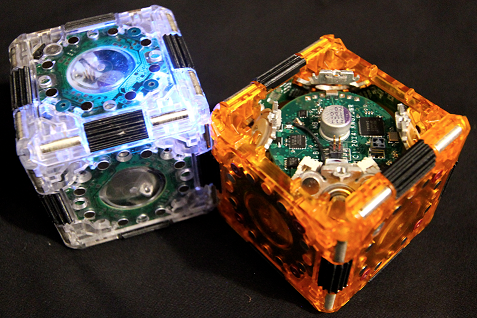
\includegraphics[width=3.4in]{Figures/cover.png}
%
%  \caption{M-Bocks modular robots with connections illuminated with onboard LEDs}
%
%  \label{fig:cover}
%\end{figure}
